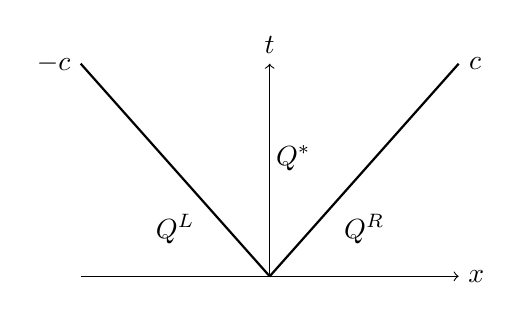
\begin{tikzpicture}[scale=0.6]
  \draw[->] (-4,0) -- (4.,0) node[right] {$x$};
  \draw[->] (0,0) -- (0,4.5) node[above] {$t$};
  \draw[thick] (0,0) -- (4.,4.5) node [right] {$c$};
  \draw[thick] (0,0) -- (-4.,4.5) node [left] {$-c$};
  \node at (2.,1.) {$\vect{Q}^R$};
  \node at (-2.,1.) {$\vect{Q}^L$};
  \node at (0.5,2.5) {$\vect{Q}^*$};
\end{tikzpicture}



%%% Local Variables:
%%% mode: latex
%%% TeX-master: "../../mainManuscript"
%%% End:
